\subsection*{\textbf{1.1 Salsa GitLab}}
\addcontentsline{toc}{subsection}{1.1 Salsa GitLab}
\vspace{-0.5cm}

Первым делом, можно зарегистрироваться в
\href{https://salsa.debian.org/public}{GitLab Salsa} --- это официальный
GitLab-сервер Debian. Там хранятся исходники пакетов, ведутся обсуждения,
принимаются merge request'ы и работает CI. Этот шаг углубит вас в мир Debian.

Можно и не регистрировать аккаунт, а придерживаться старого способа участия в
Debian, если вам так хочется:
\begin{itemize}
    \vspace{-0.3cm}
    \item отправлять патчи по email --- старый классический способ Debian;
    \item писать в BTS (bugs.debian.org);
    \item участвовать в обсуждениях.
    \vspace{-0.3cm}
\end{itemize}

Но если вы хотите участвовать в более современном формате, то лучше всё-таки
создать аккаунт в Salsa: так будет проще следить за репозиториями, отправлять
merge request'ы, участвовать в обсуждениях и пользоваться CI.

Пройдите регистрацию на \url{https://salsa.debian.org/users/sign_up}

\begin{center}
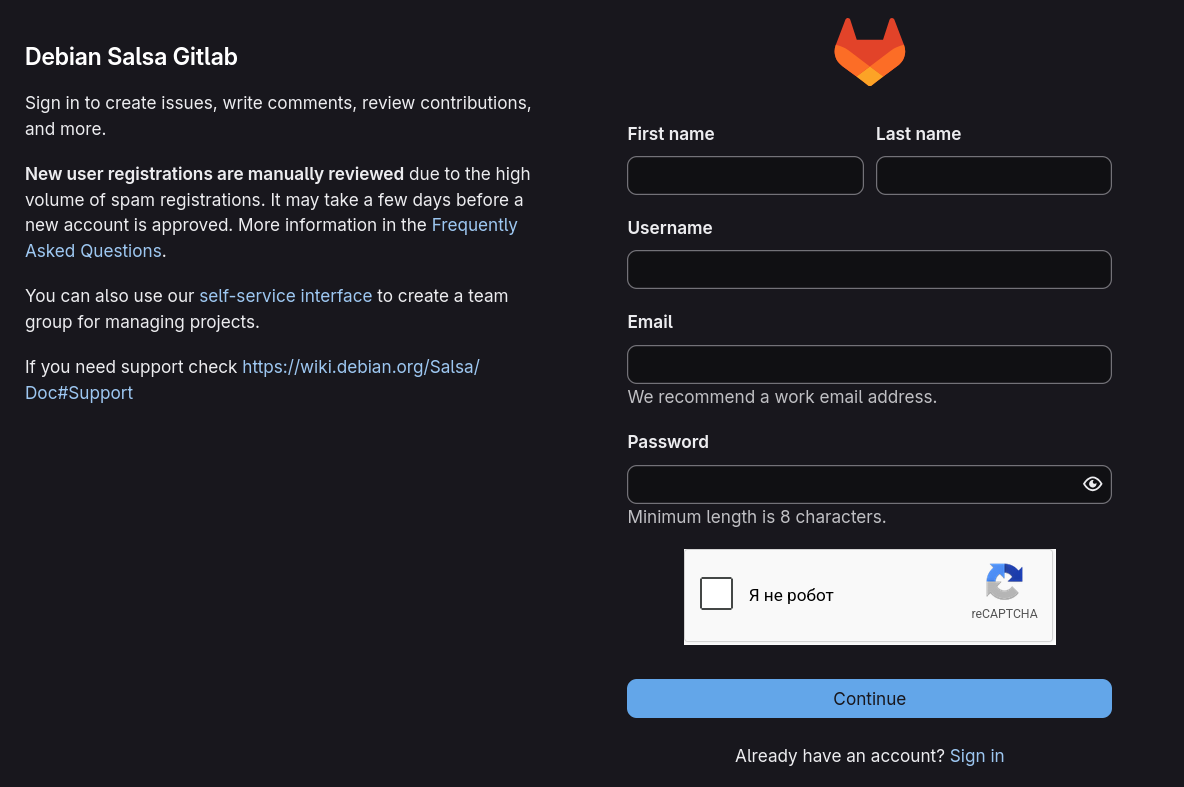
\includegraphics[width=0.70\textwidth]{images/salsa-sign-up.png}

\small \textbf{Salsa GitLab регистрация}
\vspace{-0.3cm}
\end{center}

и дождитесь, пока ваша учётная запись будет активирована (это может занять
некоторое время, наберитесь терпения).

\vspace{10cm}

После входа в аккаунт, можно добавить SSH-ключ \textbf{(Preferences ---> SSH
Keys)} --- он нужен, чтобы безопасно подключаться к GitLab и пушить/клонировать
репозитории без ввода пароля каждый раз.

\begin{center}
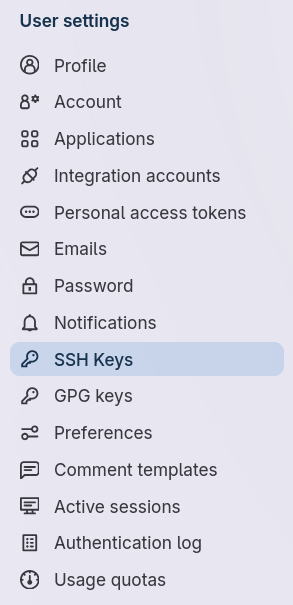
\includegraphics[width=0.20\textwidth]{images/salsa-ssh-keys.png}

\small \textbf{SSH Keys}
\vspace{-0.3cm}
\end{center}

Генерация SSH ключа происходит с помощью команды:
\vspace{-0.5cm}
\begin{verbatim}
$ ssh-keygen -f salsa
\end{verbatim}

\vspace{-0.3cm}
Скопируйте публичный ключ в буфер обмена:
\vspace{-0.5cm}
\begin{verbatim}
$ cat ~/.ssh/salsa.pub | xsel -b -i
\end{verbatim}

\vspace{-0.3cm}
Нажмите \textbf{Add new key} в GitLab и вставьте его в форму \textbf{Key}.

\textbf{Usage type: Authentication \& Signing}\\
(Authentication --- для входа/доступа по SSH)\\
(Signing --- для подписи Git-коммитов)

\textbf{Expiration date}: можете выбрать срок действия SSH-ключа. Если поставить дату,
ключ потом автоматически перестанет работать. Это полезно для безопасности. Я
обычно ставлю на 5 лет.

Удалите публичный ключ с вашего устройства:
\vspace{-0.5cm}
\begin{verbatim}
$ rm ~/.ssh/salsa.pub
\end{verbatim}

\vspace{-0.3cm}
Для безопасности проверьте, что у директории\texttt{~/.ssh} установлены права
\textbf{700}, а у приватного ключа\texttt{~/.ssh/salsa} --- \textbf{600}. Это
стандарт.

\vspace{10cm}

После того как вы настроили свой Salsa GitLab, можно немного осмотреться.

Ссылки:
\begin{itemize}
    \vspace{-0.3cm}
    \item \url{https://salsa.debian.org/public}
    \item \url{https://salsa.debian.org/explore/projects/starred}
    \vspace{-0.3cm}
\end{itemize}

\begin{center}
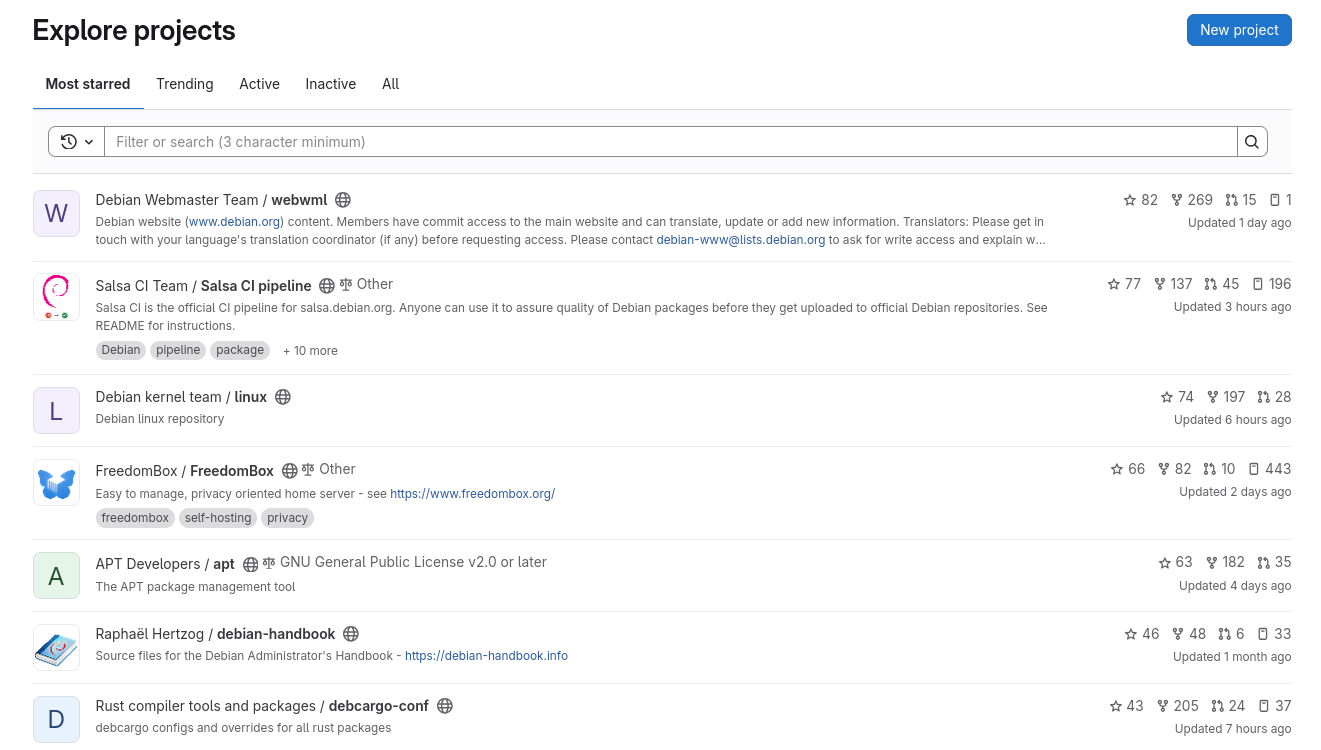
\includegraphics[width=0.95\textwidth]{images/salsa-view.png}

\small \textbf{Обзор Salsa GitLab}
\vspace{-0.3cm}
\end{center}

Думаю, вы уже заметили, что репозитории не просто разбросаны по GitLab, а
принадлежат определенным командам (Teams), которые регулярно обновляют
репозитории, исправляют баги, тестируют, делают какие-то правки и имеют
определенные привилегии в этих репозиториях. Вы можете посмотреть команды в
GitLab и увидеть, сколько репозиториев сопровождает каждая из них. Например,
если вас интересует ядро Linux в Debian, обратите внимание на
\url{https://salsa.debian.org/kernel-team}. Посмотрите на различные ветки в
репозиториях, на теги, коммиты, merge request'ы, CI и т.д.

Не пугайтесь, если чего-то не понимаете: это нормально. Сначала глаза
разбегаются, и может показаться, что всё слишком сложно, но со временем
структура репозиториев и рабочий процесс станут гораздо понятнее.

Тем более, многие инженеры в Debian работают не над всем сразу, а над
конкретными узкими задачами. Со временем перестаёшь замечать этот шум,
сосредотачиваешься на своей области, и всё становится гораздо проще. Нужно
просто занять свою нишу.

\vspace{10cm}

\subsection*{\textbf{1.2 Выбор направления и Debian Teams}}
\addcontentsline{toc}{subsection}{1.2 Выбор направления и Debian Teams}
\vspace{-0.5cm}

Давайте сначала разберёмся, как именно вы можете помочь Debian и куда можно
внести свой вклад.

Важная ссылка: \url{https://www.debian.org/intro/help.en.html}

Знайте: не все участники Debian являются разработчиками, и вам совершенно не
обязательно уметь программировать, чтобы участвовать. Есть множество способов
помочь Debian.

Если коротко, то:

1. Разработка и сопровождение пакетов.\\
   Писать программы, исправлять баги, делать патчи, сопровождать пакеты,
   заниматься безопасностью, портированием и инфраструктурой.

2. Тестирование и поиск ошибок.\\
   Проверять Debian и программы в нём, воспроизводить баги, отправлять отчёты в
   BTS, тестировать установщик и образы.

3. Документация.\\
   Писать инструкции, заметки, статьи, улучшать официальную документацию и
   Debian Wiki.

4. Переводы и локализация.\\
   Переводить программы, документацию, страницы сайта и проверять существующие
   переводы.

5. Помощь другим пользователям.\\
   Отвечать на вопросы, помогать на форумах, в Mailing Lists, IRC и других
   каналах общения.

6. Участие в мероприятиях.\\
   Помогать с DebConf, MiniDebConf, локальными встречами и другими событиями
   сообщества.

7. Пожертвования и ресурсы.\\
   Поддерживать Debian деньгами, железом, хостингом, зеркалами и другими
   ресурсами.

8. Популяризация Debian.\\
   Рассказывать о Debian, рекомендовать его другим, делать доклады, писать
   материалы, делиться опытом использования.

9. Поддержка от организаций.\\
   Компания или организация может помогать Debian ресурсами, спонсорством,
   инфраструктурой или рабочим временем сотрудников.

Задумайтесь, что вам нравится и что вам интересно в Debian. Может быть, есть
какой-то компонент, которым вы пользуетесь чаще других, и вам интересно, что в
нём происходит? Или у вас есть любимый текстовый редактор, терминал или
графическая оболочка? Может быть, вам интересны языки, и вы хотите вносить вклад
в локализацию любимых программ? Или вам хочется разбираться в CVE, тестировать
уязвимости и помогать с их исправлением? А может быть, вам интересны игры в
Debian? Или вам просто нравится главный сайт Debian, и вы хотите немного
подредактировать текст? Или вам нравится разбираться в конфигурации ядра и
улучшать её? А может, вам просто нравятся шрифты, иконки и всё такое? А может
CI? Контейнеризация? Виртуализация? Музыка/Видео? Браузер? Модули ядра?
Установщик Debian? Загрузка Debian? Перечислять можно бесконечно.

Начинать лучше с того, что вам уже нравится и чем вы сами пользуетесь: так
гораздо проще найти свою нишу, не потеряться в огромной экосистеме Debian и
постепенно превратить интерес в реальный вклад.

Например, я обожаю Vim и Xfce и использую их уже много лет. Соответственно, я
состою в Debian Vim Maintainers, делаю небольшой вклад и сопровождаю интересные
мне пакеты, а проекту Xfce по возможности помогаю через почтовую рассылку или
merge request'ы. Мне это интересно, потому что я сам активно этим пользуюсь.
